\chapter{Introduction}\label{chap:introduction}

In past decades, the rapid evolution of the high-performance computing (HPC) systems
offers growing computational capacity for the numerical simulations of various scientific fields,
where conducting a direct experiment is extremely expensive or notoriously complicated.
As the computing power of HPC systems gradually increases,
scientists can compute more complex and computationally intensive physical models such as
visualizing black holes~\cite{james2015gravitational,alberdi2019first},
simulating nuclear fusions~\cite{haines2016detailed,gaffney2019making},
studying laser-plasma interactions~\cite{meinecke2014turbulent,tzeferacos2018laboratory},
to name a few.

In order to simulate these physical phenomena,
it demands meticulously designed numerical algorithms for solving
nonlinear, multidimensional, and multi-physics equations judiciously.
Generally speaking, numerical algorithms require more computational power for better solution accuracy,
i.e., using high-resolution grid configuration.

However, the recent hardware development trend
--~the progression of the memory capacity per compute core has become gradually saturated~\cite{attig2011trends}~--
is compelling the HPC community to find more efficient ways
that can best exercise computing resources in pursuing computer simulations.
As reported in 2014~\cite{dongarra2014applied}, decreasing memory density per compute core
will be the primary limiting factor to the scalability of scientific simulation codes.

To meet this end, modern practitioners have relentlessly delved into advancing
high-arithmetic-intensity models that can increase numerical accuracy per degree of freedom
while operating with reduced memory requirements and data transfers in HPC architectures.
For example, in the computational fluid dynamics (CFD) community,
one such computing paradigm is to promote high-order methods in which high arithmetic intensity is achieved
by using an increasing number of higher-order terms.
Due to its high availability in increasing the quality of numerical solutions with fewer grid points,
high-order discrete methods for hyperbolic conservation laws have become primary themes in the CFD community.

Under the dual computational need for accuracy and stability,
the CFD community has developed high-order reconstruction and interpolation strategies
that can achieve spatially high-order
approximation.~\cite{woodward1984numerical,colella1984piecewise,liu1994weighted,jiang1996efficient,borges2008improved,castro2011high,mignone2010high,balsara2016efficient}

For example, in the Piecewise Parabolic Method (PPM)~\cite{woodward1984numerical},
the given data is considered a profile with piecewise quadratic polynomials,
ensuring third-order spatial accuracy of the PPM reconstruction/interpolation.
The PPM uses Total Variable Diminishing (TVD) slope limiters to piecewise profiles
to enhance the numerical stability in the sharp gradient regions.
The robustness and compactness of PPM attract scientists in the CFD community,
and it is considered a central ``high-order'' strategy even today.

On the other hand, the Weighted Essentially Non-Oscillatory (WENO) method~\cite{jiang1996efficient},
the improved version of the ENO method~\cite{harten1987uniformly},
takes a different route to strengthen the polynomial-based profile's stability.
The WENO method divides the given stencil into smaller sub-stencils and considers
lower-order polynomials in each sub-stencil.
Then, by taking a convex combination of each sub-polynomials with nonlinear weighting factors,
the WENO method constructs high-order, shock-capturing profiles in each stencil.
The nonlinear weights are designed in a way that converges to the linear weights in a smooth region.
(i.e., the convex combination in a smooth region is equivalent to the high-order, linear polynomial in a whole stencil)
Therefore, the WENO method can be interpreted as a piecewise profile
consists of varying degrees of polynomials depending on the local smoothness of the given data.

A recent study from Reyes et al.~\cite{reyes2018new,reyes2019variable} introduced
a new high-order reconstruction/interpolation strategy without considering the polynomial functions.
This new design concept utilizes Gaussian Process (GP) to estimate the data
at an arbitrary point in high-order accuracy instead of constructing polynomial functions.
The GP method can be combined with the WENO weighting scheme to bringing
the non-oscillatory feature of the WENO method.
The WENO-weighted GP method, called the GP-WENO method,
employs the marginal likelihood function of GP to measure the smoothness of the given data
instead of considering spatial derivatives in the conventional WENO method.
The GP-WENO method demonstrated a high-order spatial accuracy and stability with a compact structure
in the conventional finite volume discretization and
the primitive-variable-based finite difference method.

In order to achieve highly accurate numerical solutions,
the high-order temporal method must be considered alongside the spatial method
since the solution lies in a spatiotemporal plane.
Generally speaking, two different cases can be considered to determining
the order of accuracy: the leading error term from the \( p \)-th order spatial method
is dominant over the \( q \)-th order temporal error, \( \mathcal{O}(\Delta s^{p}) > \mathcal{O}(\dt^{q}) \)
or \textit{vice versa}, \( \mathcal{O} (\Delta s^{p}) < \mathcal{O}(\dt^{q}) \).
Practically, many research articles about the high-order spatial methods for solving
CFD simulation
use the mediocre low-order temporal methods combined with the high-order spatial methods.
These combinations showed a reasonable convergence rate between \( p \) and \( q \),
meaning that the spatial error is dominant over the temporal error
even with a lower order of temporal accuracy, \( q < p \).

\begin{figure}
    \centering
    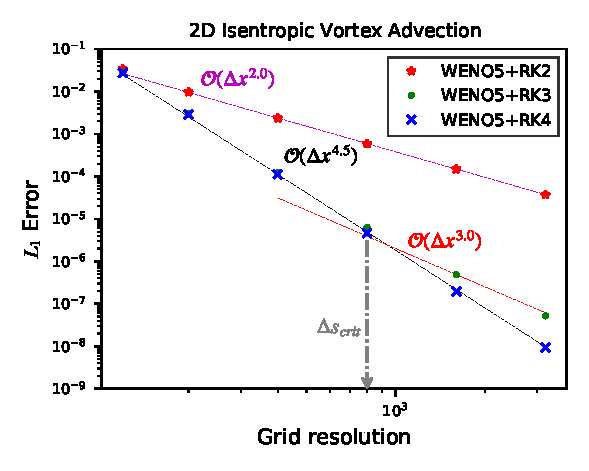
\includegraphics[width=0.85\textwidth]{fig/weno5_vortex_error_sat}
    \caption{The numerical test results for measuring errors from
        different orders of temporal methods combined with the fifth-order spatial method.
        A numerical experiment of WENO5 with RK3 exhibits
        a convergence rate degradation from a higher rate of 4.5
        following initially the fifth-order spatial accuracy of WENO5
        to a lower third-order accuracy of RK3 later on.
        In WENO5+RK4, the solution continues to converge at 4.5th order without
        a sudden drop of convergence rate. The situation is even worse for WENO5+RK2 that
        the solution over the entire range of grid resolutions is bounded to be second-order.
    }\label{fig:vortex_error_saturation}
\end{figure}
However, as reported in~\cite{lee2021recursive}, this occurrence is flipped to other ends,
i.e., temporal errors are dominant over spatial errors,
particularly in a fine grid configuration.
As shown in~\cref{fig:vortex_error_saturation}, a critical grid delta \( \Delta s_{\text{crit}} \)
exists so that the error associated with a \( q \)-th order temporal method
is comparable to and becoming dominant over the error of a \( p \)-th order spatial solver
with \( q < p \). This creates a computational dilemma of not making further enhancements
in solution accuracy, particularly when computational grids are progressively refined locally
to put more grid resolutions for improved solution quality,
such as in an adaptive mesh refinement (AMR) configuration.

Here lies the dire need for an efficient and accurate temporal scheme
in predictive science territories of CFD to acquire highly accurate numerical solutions with steadfast fidelity.
Although a method bearing high-order accuracy conveys the nexus of mathematical significance
on its right, the performance of such a high-order method should also be accompanied by computational efficiency.


For decades, multi-stage time integrators have been considered
as the standard temporal integration strategy for an extensive range of high-order numerical schemes
for partial differential equation (PDE) solvers.
Specifically, the Strong Stability Preserving Runge-Kutta (SSP-RK) method~\cite{gottlieb1998total,gottlieb2001strong,gottlieb2011strong}
is the most popular high-order time integration scheme in the CFD community.
The SSP-RK method is based on the well-known ordinary differential equation (ODE) solver,
the Runge-Kutta (RK) method, enforcing TVD property in each sub-stage of the RK method.
The SSP-RK methods have proven high fidelity and robustness
in acquiring high-order accuracy and numerical stability
in compact, straightforward numerical structures.

The number of sub-stages determines the order of accuracy of the RK method in general,
i.e., \( q \) multiple sub-stages for the \( q \)-th order RK method.
For example, the third-order RK method integrates the solution over three sub-stages.
The optimal third-order SSP-RK method also has three sub-stages with different coefficients,
which ensure the TVD property.
However, higher than third-order SSP-RK schemes require more sub-stages to achieve the TVD limitation.
It is reported in~\cite{gottlieb1998total}, the four-stage, fourth-order SSP-RK method
cannot be formulated with positive coefficients,
meaning that the classical four-stage, fourth-order RK4 is not SSP\@.
Other authors have demonstrated that SSP-RK4 with positive coefficients
could be constructed with increasing sub-stages from five up to eight~\cite{spiteri2002new,spiteri2003non},
requiring more computational costs.

Even though its portability and compactness for achieving high-order temporal accuracy,
the multi-stage time integrators are less attractive in a perspective of efficiency
due to their increasing computational costs with the order of accuracy.
For instance, the high-order spatial method and boundary conditions
should be applied at each sub-stage of the SSP-RK scheme,
which makes the overall procedure of SSP-RK computationally expensive.
In parallel simulations, these operations also increase the footprint of data movements
between node communications as the number of sub-stages grows.
This very nature of SSP-RK makes it less efficient for massively parallel simulations,
particularly when the level of adaptive mesh refinement (AMR)
progressively builds up around interesting features in simulations.

To circumvent the said issues in SSP-RK, practitioners have taken a different route
of providing a high-order temporal updating strategy for solving numerical PDEs.
The core design principle lies in formulating a conservative temporal integrator
that works for nonlinear PDEs in multiple spatial dimensions
with the equivalent high-order accuracy as in SSP-RK, but, this time, in a single-stage, single-step update.
One famous strategy is to modifying the Lax-Wendroff scheme~\cite{lax1959systems},
which uses a time-Taylor expansion of the conservative variables to achieve high-order temporal accuracy.

The effort in this direction has resulted in the Arbitrary high order DERivative (ADER) method,
which was first introduced in~\cite{toro2001towards} for linear equations.
Since then, ADER schemes have gone through several generations of a breakthrough
by numerous authors with the common goal of meeting the high-order requirement
in a compact single-step update.

The original ADER method proposed by Toro and his collaborators~\cite{toro2001towards,titarev2002ader,titarev2005ader}
achieve high-order temporal accuracy by solving a series of generalized Riemann problems (GRPs)
for temporal derivatives of the conservative variables at cell interfaces.
The temporal derivatives are obtained by applying
the so-called Lax-Wendroff or Cauchy-Kowalewski (LW/CK) procedure
similar to the original Lax-Wendroff method.
The primary purpose of the LW/CK procedure
is to convert time derivatives to spatial derivatives,
which are coupled through Jacobians and Hessians.

The ADER formulation has been further taken to a more modern direction.
Balsara et al.~\cite{balsara2009efficient} presented a new compact ADER framework
that replaced the usual Cauchy-Kowalewski procedure in the original ADER formalism
with a local continuous space-time Galerkin formulation up to fourth-order
and called the new approach ADER-CG (CG for continuous Galerkin).
The ADER-CG schemes are shown to be approximately
twice faster than the SSP-RK methods at the same order of accuracy~\cite{balsara2013efficient}.

The Picard integral formulation (PIF) method, proposed by Christlieb et al.~\cite{christlieb2015picard},
is another single-stage time integration strategy based on the Lax-Wendroff
time discretization method under the finite difference formulation.
The conventional finite difference method takes the pointwise representation of data; however,
the PIF method takes time-averaged quantities to achieve high-order temporal accuracy.
The time-averaged data is constructed through a time-Taylor expansion,
and the LW/CK procedure is used to obtain coefficients of the Taylor series.
Christlieb and his collaborators demonstrated that LW/CK procedures
could successfully be utilized for obtaining high-order terms of the numerical fluxes
for a single-stage update as in many Lax-Wendroff type works of literature.
Other studies also have shown that single-step temporal updates are more efficient
in terms of CPU time to a solution when compared to
multi-stage/multi-step methods~\cite{balsara2013efficient,lee2017piecewise,lee2021single}.

Nonetheless, single-stage time integrators are still less popular choices in the CFD community.
Designing a single-stage method generally brings more complicated and
sophisticated mathematical structures than the SSP-RK method,
requiring more implementation efforts.
A recent study from Montecinos~\cite{montecinos2020simplified} proposed
a simplification of the LW/CK procedures in the context of the implicit Taylor series.
The idea is to generalize the recursive LW/CK procedure
by considering the Jacobian matrix as a function of space and time.
The ADER-Taylor method~\cite{norman2012multi,norman2013algorithmic,norman2014weno}
is another way to reduce the number of LW/CK calculations
by adopting the Differential Transform (DT) method for high-order derivatives.

The flux Jacobians and Hessians are another implementation hurdle/bottleneck
for the Lax-Wendroff type schemes. Performing LW/CK procedures
to convert the time derivatives to spatial derivatives requires
explicit forms of the Jacobians (\( \partial_{\bU} \bF \)), Hessians (\( \partial_{\bU}^{2} \bF \)),
and higher derivatives of the flux functions (\( \partial^{k}_{\bU} \bF \))
on high-order schemes.
Finding analytical derivations of \textit{Jacobian-like} terms is
a notoriously cumbersome process, specifically for nonlinear systems.
For example, in the Euler equations, the flux Jacobians are \( 5 \times 5 \) matrices
in three spatial dimensions, and the flux Hessians are \( 5 \times 5 \times 5 \) rank three tensors.
For constructing higher than third-order temporal accuracy through the LW/CK procedure,
it is required to have analytic forms of
the third-order derivatives of the flux functions with respect to the conservative variables,
e.g., \( \partial_{\bU}^{3} \bF \).
These terms are then \( 5 \times 5 \times 5 \times 5 \) rank four tensors,
which makes the LW/CK procedure less appealing in fourth- or fifth-order temporal methods.

Another limitation on \textit{Jacobian-like} terms is the dependency on the system of equations.
Since the Jacobian-like terms are based on the flux functions of
the governing equations of the system, the hard-coded \textit{Jacobian-like} terms
should be re-derived and re-implemented whenever to change the system of equations.
For example, the high-order scheme solving Euler equations that uses \textit{Jacobian-like} terms
needs to be modified to solve other systems, such as Magnetohydrodynamics (MHD) equations.



In this regard, this dissertation develops a single-stage, high-order time integration scheme
for hyperbolic PDEs under finite difference formulation. The core design concept
is to achieve high-order accuracy within a single step
to reduce computational costs and data communications between parallel nodes.
Alongside the computational efficiency, the newly developed high-order temporal scheme is
sufficiently accurate to maintain the order of accuracy of the spatial methods,
even for the fine grid configurations.
Another important objective for designing a high-order time integrator in this dissertation is
to increase its portability. By designing a time integrator independent of the system of equations,
one can provide increased flexibility and ease of code implementation.

Consequently, a newly developed time integrator showed more than two times faster performance gain
than the conventional multi-stage methods.
Also, it can readily replace only the temporal part of any existing simulation code
independent of system of equations.
